\usetikzlibrary{shadings,shadows,shapes.arrows}

\begin{tikzpicture}
	\tikzstyle{blockstyle} = [draw,drop shadow,outer sep=3,inner sep=7,minimum size=57,line width=1, thin, draw=black!55, top color=white,bottom color=cyan,text width=70,align=center]
	
	%%%%%%%%%%%%%%
	% Left figure
	%%%%%%%%%%%%%%
	
	\def\k{0.9}
	\def\l3{-0.8}		% left x coord for 3 elements
	\def\r3{0.8}		% right x coord for 3 elements
	\node (A) at (0,3*\k) {$f(\bm u)$};
	\node[blockstyle] (B) at (0,0*\k) {$z = f(\bm x)$};
	\node (C) at (0,-3*\k) {$\bm u$};
	
	\def\uy{3.5*\k}
	\coordinate (U) at (0,\uy);
	\coordinate (V) at (0,5*\k);
	
	\path[<-] (A) edge node {} (B);
	\path[<-] (C |- B.south) edge node [right] {} (C);
	
	\draw (A) -- (U);
	\draw (U)[dashed] -- (V);
	
	\node[align=left,blue,font=\LARGE] at (0,5.5) {Forward phase};
	
	%%%%%%%%%%%%%%
	% Right figure
	%%%%%%%%%%%%%%

	\begin{scope}[xshift=135pt]
		\def\k{0.9}
		\def\l3{-0.8}		% left x coord for 3 elements
		\def\r3{0.8}		% right x coord for 3 elements
		\node (A) at (0,3*\k) {$\cfrac{\partial L}{\partial z}(\bm q)$};
		\node[blockstyle] (B) at (0,0*\k) {$z = f(\bm x)$};
		\node (C) at (0,-3*\k) {$\nabla_{\bm x}L(\bm q)$};
		
		\def\uy{3.75*\k}
		\coordinate (U) at (0,\uy);
		\coordinate (V) at (0,5*\k);
		
		\path[->] (A) edge node {} (B);
		\path[->] (C |- B.south) edge node [right] {} (C);
		
		\draw (A) -- (U);
		\draw (U)[dashed] -- (V);
		
		\node[align=left,blue,font=\LARGE] at (0,5.5) {Backward phase};
	\end{scope}

	\node[align=left,font=\large] at (2.35,-4.5) {Note:\\\;\;\;\;$\bm q=$ all the input sent to $L$};
\end{tikzpicture}
